\documentclass{article}

\usepackage[landscape, twocolumn, top=1in, bottom=0.8in, left=0.4in, right=0.4in]{geometry}

% font
\usepackage{fontspec}
\setmainfont{Georgia}[
  Path=./fonts/,
  Extension = .ttf,
  UprightFont=*-Regular,
  BoldFont=*-Bold,
  ItalicFont=*-Italic,
  BoldItalicFont=*-BoldItalic
]
\setsansfont{Metropolis}[
  Path=./fonts/,
  Extension = .ttf,
  UprightFont=*-Medium,
  BoldFont=*-Bold,
]

% utility packages
\usepackage{amsmath, amsthm, amssymb}
\usepackage{mathtools}
\usepackage[many]{tcolorbox}
\usepackage{xcolor}
\usepackage{titlesec}
\usepackage{titling}
\usepackage{enumitem}   
\usepackage{fancyhdr,lipsum}
\usepackage{float}
\usepackage{tikz}
\usepackage{enumitem}

% change font size
\usepackage[fontsize=7pt]{fontsize}

% header line
% \fancyhead[L]{\textit{06/15/2022}}
\fancyhead[R]{\textit{Duc Nguyen}}
\fancyhead[C]{{Tropical Algebra}}
\renewcommand{\headrulewidth}{0.4pt}
\renewcommand{\footrulewidth}{0pt}
\pagestyle{fancy}

% disable bibliography chapter title
% \usepackage{natbib}
% \renewcommand{\bibsection}{}

\definecolor{grey}{rgb}{0.5,0.5,0.5}
\definecolor{lightgrey}{rgb}{0.8,0.8,0.8}
\definecolor{darkgrey}{rgb}{0.3,0.3,0.3}
\definecolor{orange}{rgb}{0.94, 0.55, 0.294}
\definecolor{pink}{rgb}{0.94, 0.29, 0.7}
\definecolor{yellow}{rgb}{1, 0.749, 0}
\definecolor{green}{rgb}{0.235,0.702,0.443}
\newcommand{\chapfnt}{\fontsize{16}{19}}
\newcommand{\secfnt}{\fontsize{14}{8}}
\newcommand{\ssecfnt}{\fontsize{11}{0}}

\renewcommand{\hline}{\noindent\makebox[\linewidth]{\rule{12cm}{1pt}}}

\titleformat{\chapter}[display]
{\normalfont\chapfnt\bfseries}{\chaptertitlename\ \thechapter}{20pt}{\chapfnt}

\titleformat{\section}
{\normalfont\sffamily\secfnt\bfseries}{\thesection}{}{}

\titleformat{\subsection}
{\normalfont\sffamily\ssecfnt\mdseries}{\thesubsection}{}{}

\titleformat{\subsubsection}
{\normalfont\sffamily\fontsize{9}{0}\mdseries\color{grey}}{\thesubsection}{}{}

\titlespacing*{\chapter} {0pt}{50pt}{40pt}
\titlespacing*{\section} {0pt}{0pt}{8pt}
\titlespacing*{\subsection} {0pt}{12pt}{8pt}

\linespread{1.3}

\newtcbtheorem[auto counter,number within=section]{theorem}%
{Theorem}{
    fonttitle=\upshape, 
    fontupper=\upshape,
    boxrule=0pt,
    leftrule=3pt,
    arc=0pt,auto outer arc,
    colback=white,
    colframe=orange,
    colbacktitle=white,
    coltitle=orange,
    oversize,
    enlarge top by=1mm,
    enlarge bottom by=1mm,
    enhanced jigsaw,
    interior hidden, 
    before skip=12pt,
    overlay={
      \draw[line width=1.5pt,orange] (frame.north west) -- (frame.south west);
    }, 
    frame hidden}{theorem}
    
\newtcbtheorem[]{exercise}%
{Exercise}{
      theorem name,
    fonttitle=\upshape, 
    fontupper=\upshape,
    boxrule=0pt,
    leftrule=3pt,
    arc=0pt,auto outer arc,
    colback=white,
    colframe=pink,
    colbacktitle=white,
    coltitle=pink,
    oversize,
    enlarge top by=1mm,
    enlarge bottom by=1mm,
    enhanced jigsaw,
    interior hidden, 
    before skip=12pt,
    after skip=0pt,
    overlay={
      \draw[line width=1.5pt,pink] (frame.north west) -- (frame.south west);
    }, 
    frame hidden}{exercise}

\newtcbtheorem[auto counter,number within=section]{lemma}%
{Lemma}{
    fonttitle=\upshape, 
    fontupper=\upshape,
    boxrule=1pt,
    toprule=0pt,
    leftrule=3pt,
    arc=0pt,auto outer arc,
    colback=white,
    colframe=orange,
    colbacktitle=white,
    coltitle=orange,
    oversize,
    enlarge top by=1mm,
    enlarge bottom by=1mm,
    enhanced jigsaw,
    interior hidden, 
    before skip=12pt,
    after skip=0pt,
    overlay={
      \draw[line width=1.5pt,orange] (frame.north west) -- (frame.south west);
    }, 
    frame hidden}{lemma}
    
\newtcbtheorem[auto counter,number within=section]{example}%
{Example}{
    fonttitle=\upshape, 
    fontupper=\upshape,
    boxrule=1pt,
    toprule=0pt,
    leftrule=3pt,
    arc=0pt,auto outer arc,
    colback=white,
    colframe=green,
    colbacktitle=white,
    coltitle=green,
    oversize,
    enlarge top by=1mm,
    enlarge bottom by=1mm,
    enhanced jigsaw,
    interior hidden, 
    before skip=12pt,
    overlay={
      \draw[line width=1.5pt,green] (frame.north west) -- (frame.south west);
    }, 
    frame hidden}{example}
    
\newtcbtheorem[]{important}%
{Wichtig}{
    fonttitle=\upshape, 
    fontupper=\upshape,
    boxrule=0pt,
    leftrule=3pt,
    arc=0pt,auto outer arc,
    colback=white,
    colframe=pink,
    colbacktitle=white,
    coltitle=pink,
    oversize,
    enlarge top by=1mm,
    enlarge bottom by=1mm,
    enhanced jigsaw,
    interior hidden, 
    before skip=12pt,
    overlay={
      \draw[line width=1.5pt,pink] (frame.north west) -- (frame.south west);
    }, 
    frame hidden}{important}
    
\renewcommand{\baselinestretch}{1.4} 
\makeatletter
\let\old@rule\@rule
\def\@rule[#1]#2#3{\textcolor{lightgrey}{\old@rule[#1]{#2}{#3}}}
\makeatother


\begin{document}

\section*{Tropical Algebra}

\subsection*{A.}

\begin{itemize}
	\item \( S \subset \mathbb{R}^n \) is \textbf{\textit{tropically convex}} if \( x,y \in S \) and \( a,b \in \mathbb{R} \) implies that \( a \odot x \oplus b \odot y \in S \)
	\begin{itemize}
		\item in other words: \emph{tropical convex combinations are just tropical linear combinations}
		\item if \( S \) is tropically convex, then \( S + \mathbb{R} 1 \subset S \); hence we identify \( S \) with its image in \( \mathbb{R}^n / \mathbb{R}1 \subset \Pi \mathbb{P}^{n-1} \)
  	\item Example: \( V = \left\{ (-2,1,1), (-2,-2,-2), (-1,-1,-2), (0,0,0) \right\} \), the image of \( V \) in \( \Pi \mathbb{P}^{n-1} \) is \( \left\{ (-3,0,0), (0,0,0), (1,1, 0) \right\} \)
   
		\begin{figure}[H]
			\centering
			\includegraphics[width=5cm]{graphics/convex_hull_1.jpg}
			\caption{The tropical convex hull of \( V \)}
		\end{figure}
	\end{itemize}

	\item \textbf{\textit{Tropical polynomial function}} \( p: \mathbb{R}^n \to \mathbb{R} \) is the minimum of a finite set of linear functions 
 	\item \textbf{\textit{Hypersurface}} \( V(p) \) is the set of all points where \( p \) attains its minimum at least twice; equivalently \( p \) is not linear at \( w \)
 
\end{itemize}

\subsection*{B. Tropical Linear Algebra}

\begin{itemize}
	\item We want to compute the eigenspace of 
	\( 
		A = 
		\begin{bmatrix}
			3 & 4 & 4 \\ 4 & 3 & 4 \\ 4 & 4 & 3 
		\end{bmatrix}
	\).
	Its eigenvalue \( \lambda(A) \) is \( 3 \) because of the loop. Then, 
	\( 
		B = B^+ = B^+_0 =
		\begin{bmatrix}
			0 & 1 & 1 \\ 1 & 0 & 1 \\ 1 & 1 & 0
		\end{bmatrix}.
	\)
		The eigenspace is the image of \( B_0^+ \) under tropical arithmetic. Multiplying with the unit vectors \( e_1 = [0, \infty, \infty]^T, e_2 = [\infty, 0, \infty]^T, e_3 = [\infty, \infty, 0]^T \) from the right yields the vectors \( [0,1,1]^T, [1,0,1]^T, [1,1,0]^T \), respectively. We normalize the vectors to draw them in the projective space \( \Pi \mathbb{P}^2 \) (normalizing means to multiply each vector by a scalar such that the third coordinate vanishes). This gives us 
		\begin{align*}
			\begin{bmatrix}
				-1 \\ 0 \\ 0
			\end{bmatrix},
			\begin{bmatrix}
				0 \\ -1 \\ 0
			\end{bmatrix},
			\begin{bmatrix}
				1 \\ 1 \\ 0
			\end{bmatrix}
		\end{align*}
		Here is the picture in \( \Pi \mathbb{P}^2 \):
		\begin{figure}[H]
			\centering
			\begin{tikzpicture}
				\draw[step=1cm,gray,very thin] (-2.9,-2.9) grid (2.9,2.9);
				\filldraw[black] (-1,0) circle (2pt);
				\filldraw[black] (0,-1) circle (2pt);
				\filldraw[black] (1,1) circle (2pt);

				\filldraw[gray] (0,0) circle (2pt);
				\node[anchor=south west] at (0,0) {$(0,0)$};
			\end{tikzpicture}
		\end{figure}
		Next, we draw the tropical convex hull of these three points to obtain the image of \( B^+_0 \) in \( \Pi \mathbb{P}^2 \). The eigenspace is a hexagon
		\begin{figure}[H]
			\centering
			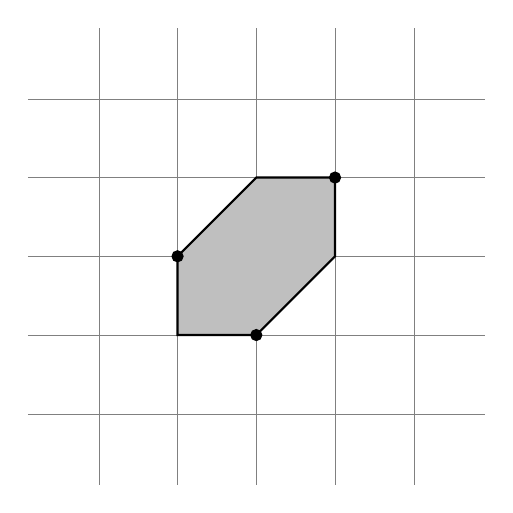
\begin{tikzpicture}
				\draw[step=1cm,gray,very thin] (-2.9,-2.9) grid (2.9,2.9);

				\filldraw[color=black, fill=black!25, thick] (-1, 0) -- (-1,-1) -- (0,-1) -- (1,0) -- (1,1) -- (0, 1) -- (-1, 0);

				\filldraw[black] (-1,0) circle (2pt);
				\filldraw[black] (0,-1) circle (2pt);
				\filldraw[black] (1,1) circle (2pt);
			\end{tikzpicture}
		\end{figure}
		Here is a computation for the convex hull of \( \left\{ [-1,0, 0]^T, [1,1,0]^T \right\} \). We want to compute \( a \odot [-1, 0, 0]^T \oplus b \odot [1,1,0]^T = [\min(a-1,b+1), \min(a, b+1), \min(a,b)]^T \) for any real scalars \( a \) and \( b \). Consider the case that the convex hull yields the point 
		\begin{align*}
			\begin{bmatrix}
				a-1 \\ a \\ b
			\end{bmatrix} \overset{\text{normalize}}{\leadsto} \begin{bmatrix}
				a-1-b \\ a-b \\ 0
			\end{bmatrix}.
		\end{align*}
		This case occurs if and only if
		\begin{align*}
			\begin{cases}
				a-1 &\leq b + 1 \\
				a 	&\leq b+1 \\
				b 	&\leq a
			\end{cases} \quad \iff \quad
			\begin{cases}
				a - 2 &\leq b \\
				a - 1 &\leq b \\
				b 		&\leq a
			\end{cases}.
		\end{align*}
		So, \( b \in [a-1, a] \). Next, by assumption we have  \( x = a - 1 - b \) and \( y = a-b \). Subtracting the first equation with the second gives \( x - y = - 1 \). Hence, \( x + 1 = y \). Since \( b \in [a-1, a] \), we obtain \( x \in [-1,0] \). With this information, we draw a line segment \( x + 1 = y \) for \( x \in [-1,0] \):
		\begin{figure}[H]
			\centering
			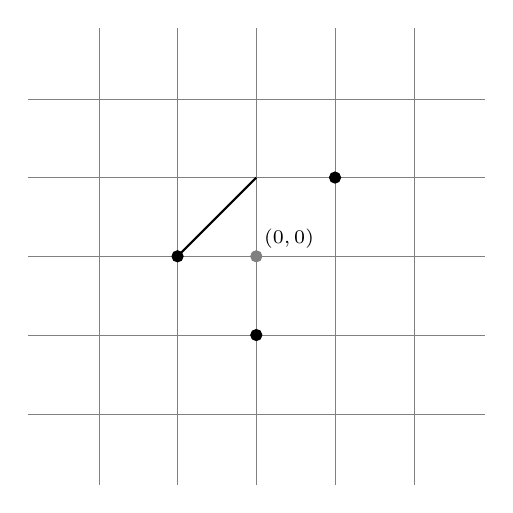
\begin{tikzpicture}
				\draw[step=1cm,gray,very thin] (-2.9,-2.9) grid (2.9,2.9);

				\filldraw[color=black, fill=black!25, thick] (-1, 0) -- (0,1);

				\filldraw[black] (-1,0) circle (2pt);
				\filldraw[black] (0,-1) circle (2pt);
				\filldraw[black] (1,1) circle (2pt);

				\filldraw[gray] (0,0) circle (2pt);
				\node[anchor=south west] at (0,0) {$(0,0)$};
			\end{tikzpicture}
		\end{figure}
		However, this does not finish the computation of the convex hull yet. We still need to consider the other cases. Some lead to contradictions, some lead to valid cases. If we compute everything correctly, we will obtain the following picture for the convex hull of \( \left\{ [-1,0, 0]^T, [1,1,0]^T \right\} \):
		\begin{figure}[H]
			\centering
			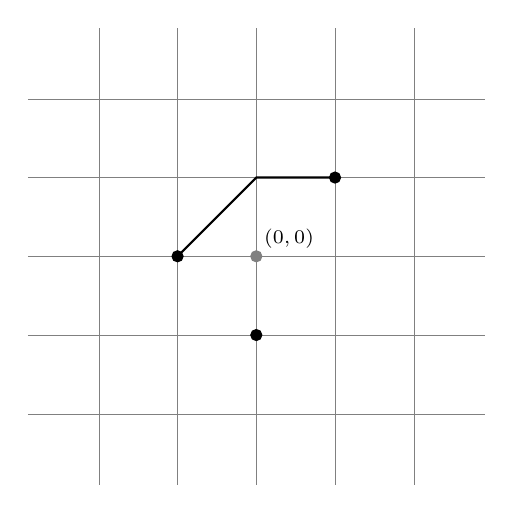
\begin{tikzpicture}
				\draw[step=1cm,gray,very thin] (-2.9,-2.9) grid (2.9,2.9);

				\draw[color=black, thick] (-1, 0) -- (0,1) -- (1,1);

				\filldraw[black] (-1,0) circle (2pt);
				\filldraw[black] (0,-1) circle (2pt);
				\filldraw[black] (1,1) circle (2pt);

				\filldraw[gray] (0,0) circle (2pt);
				\node[anchor=south west] at (0,0) {$(0,0)$};
			\end{tikzpicture}
			\caption{Convex hull of \( \left\{ [-1,0, 0]^T, [1,1,0]^T \right\} \)}
		\end{figure}
	\end{itemize}
\end{document}